\documentclass[a4paper,12pt]{article}
\usepackage[framed,numbered,autolinebreaks,useliterate]{mcode}
\usepackage{CJKutf8}
\setlength{\headheight}{15pt} 
\usepackage{textcomp}
\usepackage{amsmath}
\usepackage{amssymb}
\usepackage{listings}
\usepackage{float}
\usepackage{xcolor}
\usepackage{color}
\usepackage{fancyhdr}
\usepackage{lastpage}
\usepackage{times}
\usepackage{mathptmx}
\usepackage{geometry}
\usepackage{booktabs}
\usepackage{graphicx}
\geometry{left=3.17cm,right=3.17cm,top=2.54cm,bottom=2.54cm}
\usepackage{indentfirst}
\setlength{\parindent}{0em}



\begin{document}
\begin{CJK*}{UTF8}{gbsn}



\section{实验课题}
常见平面图形的面积计算, 要求绘制出函数的图形, 计算图形封闭部分的面积.
\begin{enumerate}
\item 三叶玫瑰线$r=a\sin{3\theta}(a=3)$.
\item 四叶玫瑰线$r=a\cos{2\theta}(a=4)$.
\item 六叶玫瑰线$r=a\cos^2{3\theta}(a=2)$.
\item 双纽线$r^2=a^2\cos{2\theta}(a=2)$.
\item 笛卡尔叶形线.$x^3+y^3=3axy(a=2)$.
\end{enumerate}



\section{三叶玫瑰线}
首先, 在极坐标系下画出三叶玫瑰线的图像, 程序如下:\vspace{-15pt}
\begin{lstlisting}
rho = 3 * sin(3*theta);
polar(theta,rho);
\end{lstlisting}\par\vspace{10pt}
\textbf{图1}是用\textsc{Matlab}绘制出的三叶玫瑰线图形.\vspace{-5pt}
\begin{center}
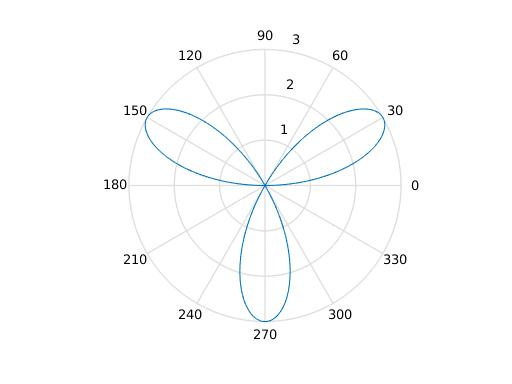
\includegraphics[width = 10cm]{three_leaf_rose_curve.jpg}\\
\vspace{-15pt}\textbf{图1} 三叶玫瑰线\\
\end{center}\vspace{5pt}
接着, 求三叶玫瑰线闭合部分的面积, 该面积的表达式为
\begin{equation*}
S_1=3\int_{0}^{\pi/3}\int_{0}^{a\sin{3\theta}}r{\rm d}r{\rm d}\theta.
\end{equation*}
计算面积的\textsc{Matlab}程序如下, 最终得到的计算结果是$\pi a^2/4$.\vspace{-15pt}
\begin{lstlisting}
S1 = 3 * int(int(r,r,0,a*sin(3*s)),s,0,pi/3);
\end{lstlisting}\par



\section{四叶玫瑰线}
首先, 在极坐标系下画出四叶玫瑰线的图像, 程序如下:\vspace{-15pt}
\begin{lstlisting}
rho = 4 * cos(2*theta);
polar(theta,rho);
\end{lstlisting}\par\vspace{10pt}
\textbf{图2}是用\textsc{Matlab}绘制出的四叶玫瑰线图形.\vspace{-5pt}
\begin{center}
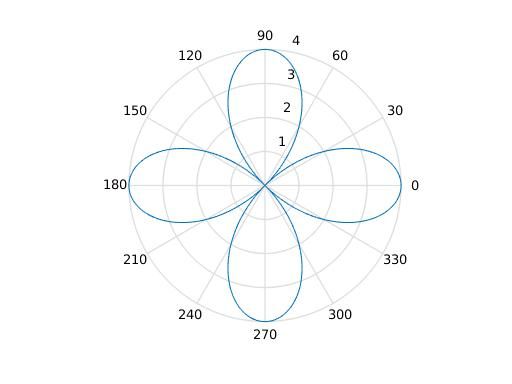
\includegraphics[width = 10cm]{four_leaf_rose_curve.jpg}\\
\vspace{-15pt}\textbf{图2} 四叶玫瑰线\\
\end{center}\vspace{5pt}
接着, 求四叶玫瑰线闭合部分的面积, 该面积的表达式为
\begin{equation*}
S_2=4\int_{-\pi/4}^{\pi/4}\int_{0}^{a\cos{2\theta}}r{\rm d}r{\rm d}\theta.
\end{equation*}
计算面积的\textsc{Matlab}程序如下, 最终得到的计算结果是$\pi a^2/2$.\vspace{-15pt}
\begin{lstlisting}
S2 = 4 * int(int(r,r,0,a*cos(2*s)),s,-pi/4,pi/4);
\end{lstlisting}\par



\section{六叶玫瑰线}
首先, 在极坐标系下画出六叶玫瑰线的图像, 程序如下:\vspace{-15pt}
\begin{lstlisting}
rho = 2 * cos(3*theta).^2;
polar(theta,rho);
\end{lstlisting}\par\vspace{10pt}
\textbf{图3}是用\textsc{Matlab}绘制出的六叶玫瑰线图形.\vspace{-5pt}
\begin{center}
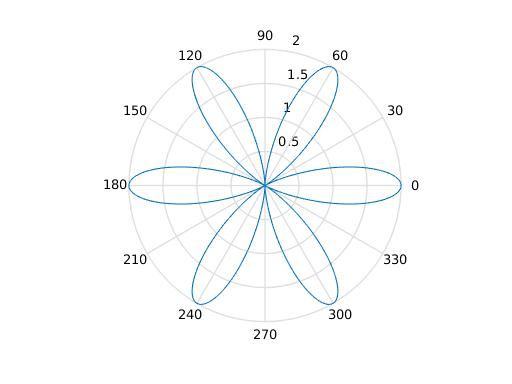
\includegraphics[width = 10cm]{six_leaf_rose_curve.jpg}\\
\vspace{-15pt}\textbf{图3} 六叶玫瑰线\\
\end{center}\vspace{5pt}
接着, 求六叶玫瑰线闭合部分的面积, 该面积的表达式为
\begin{equation*}
S_3=6\int_{-\pi/6}^{\pi/6}\int_{0}^{a\cos^2{3\theta}}r{\rm d}r{\rm d}\theta.
\end{equation*}
计算面积的\textsc{Matlab}程序如下, 最后得到的计算结果是$3\pi a^2/8$.\vspace{-15pt}
\begin{lstlisting}
S3 = 6 * int(int(r,r,0,a*cos(3*s)^2),s,-pi/6,pi/6);
\end{lstlisting}\par

\section{双纽线}
首先, 在极坐标系下画出双纽线的图像, 程序如下:\vspace{-15pt}
\begin{lstlisting}
rho = 2 * sqrt(cos(2*theta));
polar(theta,rho);
\end{lstlisting}\par\vspace{10pt}
\textbf{图4}是用\textsc{Matlab}绘制出的双纽线图形.\vspace{-5pt}
\begin{center}
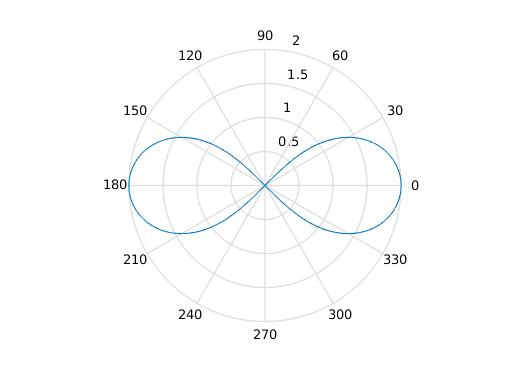
\includegraphics[width = 10cm]{lemniscate.jpg}\\
\vspace{-15pt}\textbf{图4} 双纽线\\
\end{center}\vspace{5pt}
接着, 求双纽线闭合部分的面积, 该面积的表达式为
\begin{equation*}
S_4=2\int_{-\pi/4}^{\pi/4}\int_{0}^{a\sqrt{\cos{2\theta}}}r{\rm d}r{\rm d}\theta.
\end{equation*}
计算面积的\textsc{Matlab}程序如下, 最后得到的计算结果是$a^2$.\vspace{-15pt}
\begin{lstlisting}
S4 = 2 * int(int(r,r,0,a*sqrt(cos(2*s))),s,-pi/4,pi/4);
\end{lstlisting}\par



\section{笛卡尔叶形线}
首先, 我们先用参数方程表示$x$和$y$, 参数方程如下:
\begin{equation*}
x=\frac{3at}{1+t^3}, y=\frac{3at^2}{1+t^3}.
\end{equation*}
接着我们画出笛卡尔叶形线在第一象限的图像.\vspace{-15pt}
\begin{lstlisting}
x = @(t) 6*t./(1+t.^3);
y = @(t) 6*t.^2./(1+t.^3);
t = 0:0.001:50;
plot(x(t),y(t));
\end{lstlisting}\par\vspace{10pt}
\textbf{图5}是笛卡尔叶形线的图像.\vspace{-5pt}
\begin{center}
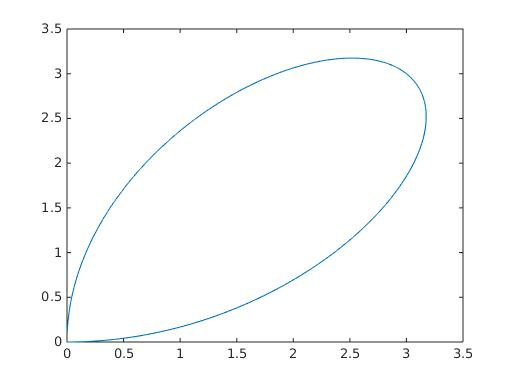
\includegraphics[width = 9cm]{descartes_folium.jpg}\\
\vspace{-10pt}\textbf{图5} 笛卡尔叶形线\\
\end{center}\vspace{5pt}
如果我们求$x(t)$的驻点可以得到$t=1/\sqrt[3]{2}$. 以这个点为分界点, 我们可以把闭合曲线分为两段处理. 所以闭合图形面积的表达式为
\begin{equation*}
S_5=\int_{\frac{1}{\sqrt[3]{2}}}^{\infty}y(t)x'(t){\rm d}t - \int_{0}^{\frac{1}{\sqrt[3]{2}}}y(t)x'(t){\rm d}t.
\end{equation*}
计算面积的\textsc{Matlab}程序如下, 最后得到的计算结果是$3a^2/2$.\vspace{-15pt}
\begin{lstlisting}
S5 = vpa(int(abs(3*a*r^2/(1+r^3)*diff(3*a*r/(1+r^3),r)),r,...
    (1/2)^(1/3),inf)-int(abs(3*a*r^2/(1+r^3)*diff(3*a*r/(1+r^3),...
    r)),r,0,(1/2)^(1/3)));
\end{lstlisting}\par



\section{实验结论}
本实验难度不大, 考察了几种曲线的图形绘制和用积分求闭合区域面积. 实验中涉及简单的坐标变换和参数替换思想, 略有趣味性.



\section{附录}
\noindent\textbf{Lab04.m} 源代码
\vspace{-10pt}
\lstset{basicstyle=\ttfamily\footnotesize,escapechar=`}
\begin{lstlisting}
%Lab04.m
clear;clc;
syms a r s;
assume(a>0);
assume(r>=0);
theta = 0:0.001:2*pi;

figure('name','Three-leaf Rose Curve');
rho = 3 * sin(3*theta);
polar(theta,rho);
S1 = 3 * int(int(r,r,0,a*sin(3*s)),s,0,pi/3);
disp('the area of three-leaf rose curve:');disp(S1);

figure('name','Four-leaf Rose Curve');
rho = 4 * cos(2*theta);
polar(theta,rho);
S2 = 4 * int(int(r,r,0,a*cos(2*s)),s,-pi/4,pi/4);
disp('the area of four-leaf rose curve:');disp(S2);

figure('name','Six-leaf Rose Curve');
rho = 2 * cos(3*theta).^2;
polar(theta,rho);
S3 = 6 * int(int(r,r,0,a*cos(3*s)^2),s,-pi/6,pi/6);
disp('the area of six-leaf rose curve:');disp(S3);

figure('name','Lemniscate');
rho = 2 * sqrt(cos(2*theta));
polar(theta,rho);
S4 = 2 * int(int(r,r,0,a*sqrt(cos(2*s))),s,-pi/4,pi/4);
disp('the area of lemniscate:');disp(S4);

figure('name','Descartes Folium');
x = @(t) 6*t./(1+t.^3);
y = @(t) 6*t.^2./(1+t.^3);
t = 0:0.001:50;
plot(x(t),y(t));
S5 = vpa(int(abs(3*a*r^2/(1+r^3)*diff(3*a*r/(1+r^3),r)),r,...
    (1/2)^(1/3),inf)-int(abs(3*a*r^2/(1+r^3)*diff(3*a*r/(1+r^3),...
    r)),r,0,(1/2)^(1/3)));
disp('the area of descartes folium:');disp(S5);
\end{lstlisting}




\end{CJK*}
\end{document}
